\documentclass[]{article}

% Import packages
\usepackage{mathtools}
\usepackage{graphicx}
\usepackage[export]{adjustbox}
\usepackage{tikz}

\usetikzlibrary{positioning,shapes,arrows}

% Page initialization
\setlength{\topmargin}{-.3 in}
\setlength{\oddsidemargin}{0in}
\setlength{\evensidemargin}{0in}
\setlength{\textheight}{9.in}
\setlength{\textwidth}{6.5in}
\pagestyle{empty}

%==============================================================%
%------------------------START-DOCUMENT------------------------%
%==============================================================%
\begin{document}

%----------------------------HEADER----------------------------%

\begin{center}
    {\Large AERO 422 Homework \#2}\\ % Homework number
    \vspace{0.2 cm}
    Instructor: Vedang Deshpande\\ % Instructor name
    \vspace{0.2 cm}
    Due: September 22, 2021 at 12:40p.m.\\ % Due date
    \vspace{0.2 cm}
    Fall 2021\\ % semester
    \vspace{0.2 cm}
    (\textbf{25 Points})\\
\end{center}

\vspace{0.2 cm}

\begin{enumerate}

    %---------------------------PROBLEM-1--------------------------%
    \item Consider the function $f(t)=te^{2t}\sin{3t}$
    \begin{enumerate}
        \item (\textbf{2 points}) Find the Laplace transform using the table. Mention which entries from the table are being used.
        \item (\textbf{1 point}) Can we use the F.V.T. to determine $f(\infty)$? Why or why not?
    \end{enumerate}
    \vspace{0.4 cm}


    %---------------------------PROBLEM-2--------------------------%
    \item Find the inverse Laplace transform using the table and partial fraction expansion. Show your work.
    \begin{enumerate}
        \item (\textbf{2 points}) $$F(s)=\frac{s+10}{s^2+2s+10}$$
        \item (\textbf{3 points}) $$F(s)=\frac{s^2+1}{s(s-1)^3}$$
    \end{enumerate}
    \vspace{0.4 cm}

    %---------------------------PROBLEM-3--------------------------%
    \item A given system is found to have a transfer function that is
    $$\frac{Y(s)}{R(s)}=\frac{10(s+2)}{s^2+8s+15}$$
    \begin{enumerate}
        \item (\textbf{3 points}) Using partial fractions, determine $y(t)$ when $r(t)$ is a unit step input. Show your work.
        \item (\textbf{1 point}) Can we use F.V.T. to find $y(\infty)$? If the answer is yes, apply F.V.T. If not, explain why.
    \end{enumerate}
    \vspace{0.4 cm}

    %---------------------------PROBLEM-4--------------------------%
    \item
    \begin{enumerate}
        \item (\textbf{3 points}) Using the convolution integral, find the step response of the system whose impulse response is given below
        \[
            h(t)=
            \begin{cases}
                te^{-t} & t \geq 0\\
                0       & t < 0
            \end{cases}
        \]
        \item (\textbf{2 points}) Now use the Laplace transform table and partial fraction expansion to find $y(t)$.
        \item (\textbf{2 points}) Apply I.V.T. and F.V.T. (if applicable) to find $y(0)$ and $y(\infty)$.
    \end{enumerate}
    \vspace{0.4 cm}

    %---------------------------PROBLEM-5--------------------------%
    \item For each of the following block diagrams, reduce the block diagram to find $T(s)$, where $T(s)$ is defined by $Y(s)=T(s)R(s)$.
    
    % define the blocks
    \tikzstyle{block} = [draw, fill=black!10, rectangle, minimum height=2.5em, minimum width=4em]
    \tikzstyle{sum} = [draw, circle, node distance=1cm]
    \tikzstyle{input} = [coordinate]
    \tikzstyle{output} = [coordinate]
    
    \begin{enumerate}
        \item (\textbf{1.5 points}) \leavevmode\vadjust{\vspace{-\baselineskip}}\newline % Part A
        % Create image of block diagram
        \begin{tikzpicture}[auto, node distance=2cm,>=latex'][h]

            % Place the blocks in desired locations
            \node [input, name=input] {};
            \node [sum, right of=input, node distance=1.5cm] (sum1) {};
            \node [block, right of=sum1, node distance=4cm] (G) {$G(s)$};
            \node [block, above of=G, node distance=1.5cm] (H1) {$H_1(s)$};
            \node [block, below of=G, node distance=1.5cm] (H2) {$H_2(s)$};
            \node [sum, right of=G, node distance=4cm] (sum2) {};
            \node [output, right of=sum2, node distance=1.5cm] (output) {};

            % Once the nodes are placed, connecting them is easy. 
            \draw [draw,->] (input) -- node[left of=input, node distance=1.2cm] {$R(s)$} node[pos=0.94] {$+$} (sum1);
            \draw [->] (sum1) -- node[name=error] {} (G);
            \draw [->] (error.east|-G) |- (H1);
            \draw [->] (G) -- node[name=y] {} node[pos=0.97,below] {$+$} (sum2);
            \draw [->] (y) |- (H2);
            \draw [->] (H2) -| node[pos=0.95] {$-$} (sum1);
            \draw [->] (H1) -| (sum2) node[pos=0.95,left] {$+$};
            \draw [draw,->] (sum2) -- node[right of=input, node distance=1.2cm] {$Y(s)$} (output);

        \end{tikzpicture}
        \vspace{0.6 cm}

        \item (\textbf{3 points}) \leavevmode\vadjust{\vspace{-\baselineskip}}\newline % Part B
        % Create image of block diagram
        \begin{tikzpicture}[auto, node distance=2cm,>=latex'][h]

            % Place the blocks in desired locations
            \node [input, name=input] {};
            \node [sum, right of=input, node distance=4cm] (sum1) {};
            \node [block, above of=sum1, node distance=1.5cm] (G1) {$G_1(s)$};
            \node [sum, right of=sum1, node distance=2cm] (sum2) {};
            \node [block, right of=sum2, node distance=2.5cm] (G2) {$G_2(s)$};
            \node [block, below of=G2, node distance=1.5cm] (H1) {$H_1(s)$};
            \node [sum, left of=H1, node distance=2.5cm] (sum3) {};
            \node [block, below of=H1, node distance=1.5cm] (H2) {$H_2(s)$};
            \node [output, right of=G2, node distance=4cm] (output) {};

            % Once the nodes are placed, connecting them is easy. 
            \draw [->] (input) -- node[name=r] {} node[left of=input, node distance=2.5cm] {$R(s)$} node[pos=0.97] {$+$} (sum1);
            \draw [->] (r.east|-sum1) |- (G1);
            \draw [->] (sum1) -- node[pos=0.95,below] {$+$} (sum2);
            \draw [->] (G1) -| node[pos=0.97,left] {$+$} (sum2);
            \draw [->] (sum2) -- (G2);
            \draw [->] (G2) -- node[name=y] {} node[right of=input, node distance=2.2cm] {$Y(s)$} (output);
            \draw [->] (y) |- (H1);
            \draw [->] (y) |- (H2);
            \draw [->] (H1) -- node[pos=0.95,above] {$+$} (sum3);
            \draw [->] (H2) -| node[pos=0.97,right] {$-$} (sum3);
            \draw [->] (sum3) -| node[pos=0.97,left] {$-$} (sum1);

        \end{tikzpicture}
        \vspace{0.6 cm}

        \item (\textbf{1.5 points}) \leavevmode\vadjust{\vspace{-\baselineskip}}\newline \\ \\ % Part C
        % Create image of block diagram
        \begin{tikzpicture}[auto, node distance=2cm,>=latex'][h]

            % Place the blocks in desired locations
            \node [input, name=input] {};
            \node [block, right of=input, node distance=4cm] (G1) {$G_1(s)$};
            \node [sum, right of=G1, node distance=2.25cm] (sum1) {};
            \node [block, right of=sum1, node distance=2.25cm] (G2) {$G_2(s)$};
            \node [sum, right of=G2, node distance=2.25cm] (sum2) {};
            \node [output, right of=sum2, node distance=1.75cm] (output) {};

            % Once the nodes are placed, connecting them is easy. 
            \draw [draw,->] (input) -- node[left of=input, node distance=2.25cm] {$R(s)$} node[name=r] {} node[name=j1, below of=r, node distance=1.5cm] {} (G1);
            \draw [->] (G1) -- node[pos=0.92,above] {$+$} (sum1);
            \draw (r) |- (j1.center);
            \draw [->] (j1.center) -| node[pos=0.95,left] {$+$} (sum1);
            \draw [->] (sum1) -- (G2);
            \draw [->] (G2) -- node[pos=0.92,above] {$+$} (sum2);
            \draw [->] (j1.center) -| node[pos=0.95,left] {$+$} (sum2);
            \draw [draw,->] (sum2) -- node[right of=input, node distance=1.3cm] {$Y(s)$} (output);

        \end{tikzpicture}
        \vspace{0.6 cm}

    \end{enumerate}

\end{enumerate}

% insert image
\begin{figure}[h]
    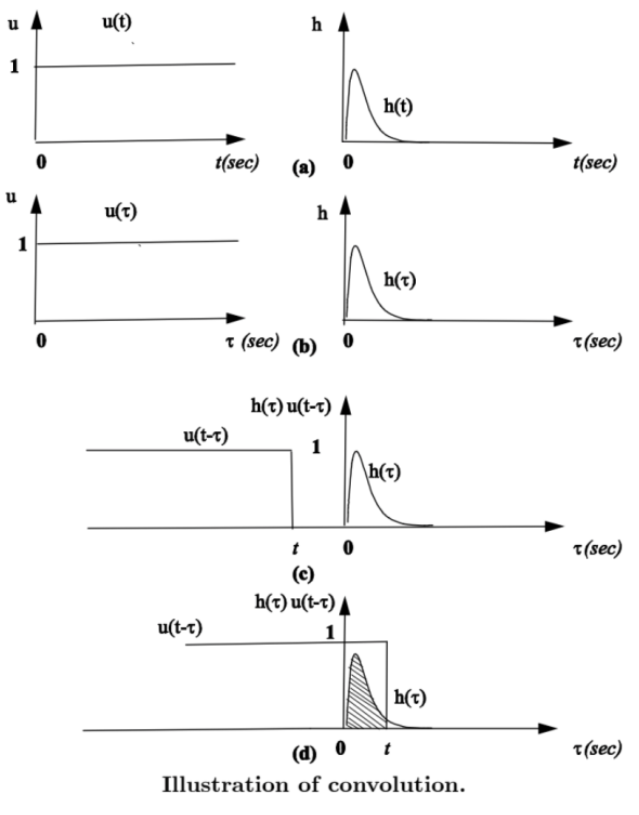
\includegraphics[scale=0.53,center]{AERO_422_HW2_image.PNG}
    \caption{Convolution integral (reference for problem 4)}
\end{figure}

\end{document}


